\documentclass[tikz,border=10pt]{standalone}
\usepackage{tikz}
\usepackage{xcolor}
\usepackage[T1]{fontenc}
\usepackage{lmodern}
\usetikzlibrary{arrows.meta,calc}

\definecolor{curBg}{RGB}{219,234,254}
\definecolor{curBdr}{RGB}{96,165,250}
\definecolor{incBg}{RGB}{254,243,199}
\definecolor{incBdr}{RGB}{251,191,36}
\definecolor{reordBg}{RGB}{254,226,226}
\definecolor{reordBdr}{RGB}{239,68,68}
\definecolor{cellBg}{RGB}{245,245,245}
\definecolor{cellBdr}{RGB}{185,185,185}

\begin{document}
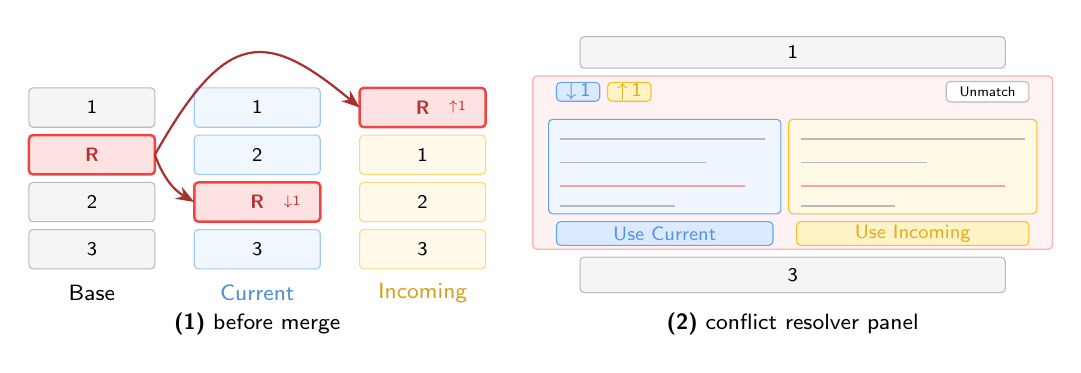
\begin{tikzpicture}[font=\sffamily\small, >=Stealth]

%%=============================================================
%% FIGURE 1 — notebook stacks before merge
%% Cell: w=1.6  h=0.5  gap=0.1
%% Column left-x:  Base=0  Current=2.1  Incoming=4.2
%% Cell top-y:  p1=3.2  p2=2.6  p3=2.0  p4=1.4 (shifted -0.3)
%% Center-y:    p1=2.95 p2=2.35 p3=1.75 p4=1.15
%% Column labels BELOW at y=0.6 — arrows route freely above at y=3.7
%%=============================================================

%% ─ BASE: [1, R, 2, 3] ─
\draw[fill=cellBg, draw=cellBdr, rounded corners=1.5pt]
    (0,2.7) rectangle (1.6,3.2);
\node[font=\sffamily\scriptsize] at (0.8,2.95) {1};

\draw[fill=reordBg, draw=reordBdr, line width=0.9pt, rounded corners=1.5pt]
    (0,2.1) rectangle (1.6,2.6);
\node[font=\sffamily\scriptsize\bfseries, color=reordBdr!75!black] at (0.8,2.35) {R};

\draw[fill=cellBg, draw=cellBdr, rounded corners=1.5pt]
    (0,1.5) rectangle (1.6,2.0);
\node[font=\sffamily\scriptsize] at (0.8,1.75) {2};

\draw[fill=cellBg, draw=cellBdr, rounded corners=1.5pt]
    (0,0.9) rectangle (1.6,1.4);
\node[font=\sffamily\scriptsize] at (0.8,1.15) {3};

%% ─ CURRENT: [1, 2, R, 3] ─
\draw[fill=curBg!40, draw=curBdr!60, rounded corners=1.5pt]
    (2.1,2.7) rectangle (3.7,3.2);
\node[font=\sffamily\scriptsize] at (2.9,2.95) {1};

\draw[fill=curBg!40, draw=curBdr!60, rounded corners=1.5pt]
    (2.1,2.1) rectangle (3.7,2.6);
\node[font=\sffamily\scriptsize] at (2.9,2.35) {2};

\draw[fill=reordBg, draw=reordBdr, line width=0.9pt, rounded corners=1.5pt]
    (2.1,1.5) rectangle (3.7,2.0);
\node[font=\sffamily\scriptsize\bfseries, color=reordBdr!75!black] at (2.9,1.75) {R};
\node[font=\sffamily\tiny, color=reordBdr!80!black, anchor=west] at (3.1,1.75) {$\downarrow$1};

\draw[fill=curBg!40, draw=curBdr!60, rounded corners=1.5pt]
    (2.1,0.9) rectangle (3.7,1.4);
\node[font=\sffamily\scriptsize] at (2.9,1.15) {3};

%% ─ INCOMING: [R, 1, 2, 3] ─
\draw[fill=reordBg, draw=reordBdr, line width=0.9pt, rounded corners=1.5pt]
    (4.2,2.7) rectangle (5.8,3.2);
\node[font=\sffamily\scriptsize\bfseries, color=reordBdr!75!black] at (5.0,2.95) {R};
\node[font=\sffamily\tiny, color=reordBdr!80!black, anchor=west] at (5.2,2.95) {$\uparrow$1};

\draw[fill=incBg!40, draw=incBdr!60, rounded corners=1.5pt]
    (4.2,2.1) rectangle (5.8,2.6);
\node[font=\sffamily\scriptsize] at (5.0,2.35) {1};

\draw[fill=incBg!40, draw=incBdr!60, rounded corners=1.5pt]
    (4.2,1.5) rectangle (5.8,2.0);
\node[font=\sffamily\scriptsize] at (5.0,1.75) {2};

\draw[fill=incBg!40, draw=incBdr!60, rounded corners=1.5pt]
    (4.2,0.9) rectangle (5.8,1.4);
\node[font=\sffamily\scriptsize] at (5.0,1.15) {3};

%% Column labels below the stacks
\node[font=\sffamily\footnotesize] at (0.8,0.6) {Base};
\node[font=\sffamily\footnotesize, color=curBdr!85!black]  at (2.9,0.6) {Current};
\node[font=\sffamily\footnotesize, color=incBdr!85!black] at (5.0,0.6) {Incoming};

%% Arrow: Base-R -> Current-R  (moved down 1 position, ↓1)
% Both arrows now originate from the right edge of Base R (x=1.6, y=2.35)
% Down arrow: Base-R -> Current-R (moved down 1 position, ↓1)
\draw[->, color=reordBdr!70!black, line width=0.8pt]
    (1.6,2.35) to[bend right=20] (2.1,1.75);
% (arrow label removed)

% Arrow: Base-R -> Incoming-R  (moved up 1 position, ↑1)
% Now starts at right edge of Base R (1.6,2.35), curves high above Current, then down to left of Incoming R
\draw[->, color=reordBdr!70!black, line width=0.8pt]
    (1.6,2.35)
    .. controls (2.5,3.95) and (3.0,3.95) .. (4.2,2.95);
% (arrow label removed)

%% Caption
\node[font=\sffamily\footnotesize, align=center] at (2.9,0.2)
    {\textbf{(1)}\ before merge};

%%=============================================================
%% FIGURE 2 — conflict resolver (essential elements only)
%% Panel x: 6.6 .. 12.8   left-col mid=8.075   right-col mid=11.225
%% Context (cell 1):  y = 3.45 .. 3.85 (shifted -0.6)
%% Action bar:        y = 2.95 .. 3.35 (shifted -0.6)
%% Conflict cells:    y = 1.6  .. 2.8  (shifted -0.6)
%% Resolution bar:    y = 1.2  .. 1.5  (shifted -0.6)
%% Context (cell 3):  y = 0.6  .. 1.05 (shifted -0.6)
%%=============================================================

%% ─ Context row above: cell 1 (identical, no conflict) ─
\draw[fill=cellBg, draw=cellBdr, rounded corners=1.5pt]
    (7.0,3.45) rectangle (12.4,3.85);
\node[font=\sffamily\scriptsize] at (9.7,3.65) {1};

%% ─ Action bar ─ (background spans down to bottom of resolution panel)
\draw[fill=reordBg!45, draw=reordBdr!40, rounded corners=1.5pt, line width=0.5pt]
    (6.4,1.15) rectangle (13,3.35);

%% Badge ↓1  (current moved down 1 position)
\draw[fill=curBg, draw=curBdr, rounded corners=1.5pt]
    (6.7,3.03) rectangle (7.25,3.27);
\node[font=\sffamily\scriptsize, color=curBdr!90!black] at (6.975,3.15) {$\downarrow$\,1};

%% Badge ↑1  (incoming moved up 1 position)
\draw[fill=incBg, draw=incBdr, rounded corners=1.5pt]
    (7.35,3.03) rectangle (7.9,3.27);
\node[font=\sffamily\scriptsize, color=incBdr!90!black] at (7.625,3.15) {$\uparrow$\,1};

%% Unmatch button
\draw[fill=white, draw=cellBdr, rounded corners=1.5pt]
    (11.65,3.02) rectangle (12.7,3.28);
\node[font=\sffamily\tiny] at (12.175,3.15) {Unmatch};

%% ─ Conflict cell columns (clearly below the action bar) ─
\draw[fill=curBg!45, draw=curBdr, rounded corners=1.5pt]
    (6.6,1.6) rectangle (9.55,2.8);

\draw[fill=incBg!45, draw=incBdr, rounded corners=1.5pt]
    (9.65,1.6) rectangle (12.8,2.8);

%% Squiggles inside left cell (suggesting code lines)
\draw[cellBdr,      line width=0.55pt] (6.75,2.55) -- (9.35,2.55);
\draw[cellBdr,      line width=0.55pt] (6.75,2.25) -- (8.6,2.25);
\draw[reordBdr!50,  line width=0.55pt] (6.75,1.95) -- (9.1,1.95);
\draw[cellBdr,      line width=0.55pt] (6.75,1.7)  -- (8.2,1.7);

%% Squiggles inside right cell
\draw[cellBdr,      line width=0.55pt] (9.8,2.55) -- (12.65,2.55);
\draw[cellBdr,      line width=0.55pt] (9.8,2.25) -- (11.4,2.25);
\draw[reordBdr!50,  line width=0.55pt] (9.8,1.95) -- (12.4,1.95);
\draw[cellBdr,      line width=0.55pt] (9.8,1.7)  -- (11.0,1.7);

%% ─ Resolution bar ─
\draw[fill=curBg, draw=curBdr, rounded corners=1.5pt]
    (6.7,1.2) rectangle (9.45,1.5);
\node[font=\sffamily\scriptsize, color=curBdr!90!black] at (8.075,1.35) {Use Current};

\draw[fill=incBg, draw=incBdr, rounded corners=1.5pt]
    (9.75,1.2) rectangle (12.7,1.5);
\node[font=\sffamily\scriptsize, color=incBdr!90!black] at (11.225,1.35) {Use Incoming};

%% ─ Context row below: cell 3 (identical, no conflict) ─
\draw[fill=cellBg, draw=cellBdr, rounded corners=1.5pt]
    (7.0,0.6) rectangle (12.4,1.05);
\node[font=\sffamily\scriptsize] at (9.7,0.825) {3};

%% Caption
\node[font=\sffamily\footnotesize, align=center] at (9.7,0.2)
    {\textbf{(2)}\ conflict resolver panel};

\end{tikzpicture}
\end{document}
